%%%%%%%%%%%%%%%%%%%%%%%%%%%%%%%%%%%%%%%%%
% Bachelor/Master Thesis 
% LaTeX Template
% Version 2.5 (27/8/17)
%
% This template was downloaded from:
% http://www.LaTeXTemplates.com
%
% Version 2.x major modifications by:
% Vel (vel@latextemplates.com)
%
% This template is based on a template by:
% Steve Gunn (http://users.ecs.soton.ac.uk/srg/softwaretools/document/templates/)
% Sunil Patel (http://www.sunilpatel.co.uk/thesis-template/)
%
% Template license:
% CC BY-NC-SA 3.0 (http://creativecommons.org/licenses/by-nc-sa/3.0/)
%
%%%%%%%%%%%%%%%%%%%%%%%%%%%%%%%%%%%%%%%%%

%----------------------------------------------------------------------------------------
%	PACKAGES AND OTHER DOCUMENT CONFIGURATIONS
%----------------------------------------------------------------------------------------

\documentclass[
11pt, % The default document font size, options: 10pt, 11pt, 12pt
%oneside, % Two side (alternating margins) for binding by default, uncomment to switch to one side
english, % ngerman for German
singlespacing, % Single line spacing, alternatives: onehalfspacing or doublespacing
%draft, % Uncomment to enable draft mode (no pictures, no links, overfull hboxes indicated)
%nolistspacing, % If the document is onehalfspacing or doublespacing, uncomment this to set spacing in lists to single
%liststotoc, % Uncomment to add the list of figures/tables/etc to the table of contents
%toctotoc, % Uncomment to add the main table of contents to the table of contents
%parskip, % Uncomment to add space between paragraphs
%nohyperref, % Uncomment to not load the hyperref package
headsepline, % Uncomment to get a line under the header
%chapterinoneline, % Uncomment to place the chapter title next to the number on one line
%consistentlayout, % Uncomment to change the layout of the declaration, abstract and acknowledgements pages to match the default layout
% oneside % to avoid doublepage
]{BachelorMasterThesis} % The class file specifying the document structure

\usepackage[utf8]{inputenc} % Required for inputting international characters
\usepackage[T1]{fontenc} % Output font encoding for international characters

\usepackage{mathpazo} % Use the Palatino font by default
% \usepackage[backend=bibtex,style=authoryear,natbib=true]{biblatex} % Use the bibtex backend with the authoryear citation style (which resembles APA)

% \addbibresource{main.bib} % The filename of the bibliography

\usepackage[autostyle=true]{csquotes} % Required to generate language-dependent quotes in the bibliography
\usepackage{amsmath}
%----------------------------------------------------------------------------------------
%	MARGIN SETTINGS
%----------------------------------------------------------------------------------------

\geometry{
	paper=a4paper, % Change to letterpaper for US letter
	inner=2.5cm, % Inner margin
	outer=3.8cm, % Outer margin
	bindingoffset=.5cm, % Binding offset
	top=1.5cm, % Top margin
	bottom=1.5cm, % Bottom margin
	%showframe, % Uncomment to show how the type block is set on the page
}

%----------------------------------------------------------------------------------------
%	THESIS INFORMATION
%----------------------------------------------------------------------------------------

\thesistitle{Multi-camera visual collision avoidance for micro aerial vehicles} % Your thesis title, this is used in the title and abstract, print it elsewhere with \ttitle
\supervisor{Ing. Matouš \textsc{Vrba}} % Your supervisor's name, this is used in the title page, print it elsewhere with \supname
\examiner{} % Your examiner's name, this is not currently used anywhere in the template, print it elsewhere with \examname
\degree{Bachelor of Science} % Your degree name, this is used in the title page and abstract, print it elsewhere with \degreename
\author{Mykola \textsc{Morhunenko}} % Your name, this is used in the title page and abstract, print it elsewhere with \authorname
\addresses{} % Your address, this is not currently used anywhere in the template, print it elsewhere with \addressname

\subject{Robotics, Computer Science} % Your subject area, this is not currently used anywhere in the template, print it elsewhere with \subjectname
\keywords{} % Keywords for your thesis, this is not currently used anywhere in the template, print it elsewhere with \keywordnames
\university{\href{https://ucu.edu.ua}{Ukrainian Catholic University}} % Your university's name and URL, this is used in the title page and abstract, print it elsewhere with \univname
\department{\href{https://apps.ucu.edu.ua}{Department of Computer Sciences}} % Your department's name and URL, this is used in the title page and abstract, print it elsewhere with \deptname
\group{\href{https://apps.ucu.edu.ua/computer-science/}{Faculty of Applied Sciences}} % Your research group's name and URL, this is used in the title page, print it elsewhere with \groupname
\faculty{\href{https://apps.ucu.edu.ua}{Faculty of Applied Sciences}} % Your faculty's name and URL, this is used in the title page and abstract, print it elsewhere with \facname

\AtBeginDocument{
\hypersetup{pdftitle=\ttitle} % Set the PDF's title to your title
\hypersetup{pdfauthor=\authorname} % Set the PDF's author to your name
\hypersetup{pdfkeywords=\keywordnames} % Set the PDF's keywords to your keywords
}

\begin{document}

\frontmatter % Use roman page numbering style (i, ii, iii, iv...) for the pre-content pages

\pagestyle{plain} % Default to the plain heading style until the thesis style is called for the body content

%----------------------------------------------------------------------------------------
%	TITLE PAGE
%----------------------------------------------------------------------------------------

\begin{titlepage}
\begin{center}

\vspace*{.06\textheight}
{\scshape\LARGE \univname\par}\vspace{1.5cm} % University name
\textsc{\Large Bachelor Thesis}\\[0.5cm] % Thesis type

\HRule \\[0.4cm] % Horizontal line
{\huge \bfseries \ttitle\par}\vspace{0.4cm} % Thesis title
\HRule \\[1.5cm] % Horizontal line
 
\begin{minipage}[t]{0.4\textwidth}
\begin{flushleft} \large
\emph{Author:}\\
\authorname % Author name - remove the \href bracket to remove the link
\end{flushleft}
\end{minipage}
\begin{minipage}[t]{0.4\textwidth}
\begin{flushright} \large
\emph{Supervisor:} \\
\href{http://mrs.felk.cvut.cz/members/phdstudents/matous-vrba}{\supname} % Supervisor name - remove the \href bracket to remove the link  
\end{flushright}
\end{minipage}\\[3cm]
 
\vfill

\large \textit{A thesis submitted in fulfillment of the requirements\\ for the degree of \degreename}\\[0.3cm] % University requirement text
\textit{in the}\\[0.4cm]
\groupname\\\deptname\\[2cm] % Research group name and department name
 
\vfill

\includegraphics[height=5cm]{UCU-Apps.png} % University/department logo - uncomment to place it

\vfill
{\large \vspace{-0.5cm} Lviv 2022}\\[4cm] % Date
 
\vfill
\end{center}
\end{titlepage}

%----------------------------------------------------------------------------------------
%	DECLARATION PAGE
%----------------------------------------------------------------------------------------

\begin{declaration}
\addchaptertocentry{\authorshipname} % Add the declaration to the table of contents
\noindent I, \authorname, declare that this thesis titled, \enquote{\ttitle} and the work presented in it are my own. I confirm that:

\begin{itemize} 
\item This work was done wholly or mainly while in candidature for a research degree at this University.
\item Where any part of this thesis has previously been submitted for a degree or any other qualification at this University or any other institution, this has been clearly stated.
\item Where I have consulted the published work of others, this is always clearly attributed.
\item Where I have quoted from the work of others, the source is always given. With the exception of such quotations, this thesis is entirely my own work.
\item I have acknowledged all main sources of help.
\item Where the thesis is based on work done by myself jointly with others, I have made clear exactly what was done by others and what I have contributed myself.\\
\end{itemize}
 
\noindent Signed:\\
\rule[0.5em]{25em}{0.5pt} % This prints a line for the signature
 
\noindent Date:\\
\rule[0.5em]{25em}{0.5pt} % This prints a line to write the date
\end{declaration}

\cleardoublepage

%----------------------------------------------------------------------------------------
%	QUOTATION PAGE
%----------------------------------------------------------------------------------------

\vspace*{0.2\textheight}

\noindent\enquote{\itshape Science, my lad, is made up of mistakes, but they are mistakes which it is useful to make, because they lead little by little to the truth.}\bigbreak

\hfill Jules Verne

%----------------------------------------------------------------------------------------
%	ABSTRACT PAGE
%----------------------------------------------------------------------------------------

\begin{abstract}
\addchaptertocentry{\abstractname} % Add the abstract to the table of contents

We live in a twenty first century - time of extremely fast developing of all electronic devices. Each month we see some brake-through in such directions as microchips modeling, flying vehicles developing, quantum computing and space exploration, bioengineering and medicine. 

in the thesis I would like to focus on micro aerial vehicles as one of the most perspective development directions and interesting personally for me. During my internship in the MRS Group I was working a lot with computer vision, and I see it as quite promising direction.

Specifically, visual collision avoidance is one of the relevant topics that is being actively researched nowadays. Drones with this feature becomes more preferable - they are safer, can last longer and easier to control. Visual collision avoidance is much less expensive than Lidars.

:TODO
\end{abstract}

%----------------------------------------------------------------------------------------
%	ACKNOWLEDGEMENTS
%----------------------------------------------------------------------------------------

\begin{acknowledgements}
\addchaptertocentry{\acknowledgementname} % Add the acknowledgements to the table of contents

I would like to thank my supervisor Ing. Matouš Vrba and all CTU MRS Group for the opportunity to have an internship there for last one and a half year, all of them was kind, they helped me a lot with advice's and sharing their experience, CTU FEE for interesting and useful for this thesis courses. I want to admire that nothing my study will not take place without my small family - Ukrainian Catholic University, especially Applied Science Faculty, all teachers and deanery for saving all students from all the worst sides of Ukrainian education system and providing only the best quality education without corruption and plagiarism.
\\

Especially I want to thank all defenders of my Motherland, The Armed Forces of Ukraine, who protect the whole Europe during the russo-Ukraian war at the cost of their own lives to make it possible for all of us to live in peace and for me to write this thesis.
\\

Finally, I would like to thank my family who supported me during whole my life, my mother Svitlana and my father Roman.
\end{acknowledgements}

%----------------------------------------------------------------------------------------
%	LIST OF CONTENTS/FIGURES/TABLES PAGES
%----------------------------------------------------------------------------------------

\tableofcontents % Prints the main table of contents

\listoffigures % Prints the list of figures

\listoftables % Prints the list of tables

%----------------------------------------------------------------------------------------
%	ABBREVIATIONS
%----------------------------------------------------------------------------------------

\begin{abbreviations}{ll} % Include a list of abbreviations (a table of two columns)
\textbf{UAV} & \textbf{U}nmanned \textbf{A}erial \textbf{V}ehicle\\
\textbf{MAV} & \textbf{M}icro Unmanned \textbf{A}erial \textbf{V}ehicle\\
\textbf{ROS} & \textbf{R}obotic \textbf{O}perating \textbf{S}ystem\\
\textbf{DoF} & \textbf{D}egree \textbf{o}f \textbf{F}reedom\\
% \textbf{MRS} & \textbf{M}ulti \textbf{R}obot \textbf{S}ystems Group\\

\end{abbreviations}

%----------------------------------------------------------------------------------------
%	PHYSICAL CONSTANTS/OTHER DEFINITIONS
%----------------------------------------------------------------------------------------

% \begin{constants}{lr@{${}={}$}l} % The list of physical constants is a three column table

% % The \SI{}{} command is provided by the siunitx package, see its documentation for instructions on how to use it

% Speed of Light & $c_{0}$ & \SI{2.99792458e8}{\meter\per\second} (exact)\\
% %Constant Name & $Symbol$ & $Constant Value$ with units\\

% \end{constants}

%----------------------------------------------------------------------------------------
%	SYMBOLS
%----------------------------------------------------------------------------------------

\begin{symbols}{lll} % Include a list of Symbols (a three column table)

% Symbol & Name & Unit \\
$f$ & focal length & px \\
% \addlinespace % Gap to separate the Roman symbols from the Greek

% $\omega$ & angular frequency & \si{\radian} \\

\end{symbols}

%----------------------------------------------------------------------------------------
%	DEDICATION
%----------------------------------------------------------------------------------------

% \dedicatory{For/Dedicated to/To my\ldots}

%----------------------------------------------------------------------------------------
%	THESIS CONTENT - CHAPTERS
%----------------------------------------------------------------------------------------

\mainmatter % Begin numeric (1,2,3...) page numbering

\pagestyle{thesis} % Return the page headers back to the "thesis" style

% Include the chapters of the thesis as separate files from the Chapters folder
% Uncomment the lines as you write the chapters

\chapter{Introduction}
\label{chapter:intro}

Micro unmanned aerial vehicles (MAVs) recently saw a rise in usage across various fields. Drones are already wide used in cinematography\footnote{\href{https://coptrz.com/drones-in-filmmaking-the-best-drones-for-the-job/\#:~:text=How\%20drones\%20are\%20used\%20in\%20big\%2Dbudget\%20films}{Coptrz, "How drones are used in big-budget films}} and advertising\footnote{\href{https://www.bangkokpost.com/business/2124327/the-future-of-advertising-could-be-drones\#:~:text=However\%2C\%20using\%20drones\%20is\%20a,automobile\%20shows\%20and\%20other\%20campaigns.}{Bangkokpost, "The future of advertising could be drones"}}, In Ukraine they are very helpful in farming (to apply pesticides to fields)\footnote{\href{https://techukraine.org/portfolio/droneua-solution-of-field-cultivation-by-drones-up-to-1-million-hectares-in-ukraine/\#:~:text=Since\%202019\%2C\%20spraying\%20drones\%20began,not\%20depend\%20on\%20soil\%20moisture.}{DroneUA}}. City emergency departments use UAVs  - firefighters can use them to see and evaluate the situation from the sky, localise the source of fire and deal with that\footnote{\href{https://www.dslrpros.com/firefighting-drones.html}{Fire Fighting Drones}}, sometimes it even can have some fire-extinguishing capsules as projectiles\footnote{\href{https://ieeexplore.ieee.org/stamp/stamp.jsp?arnumber=9328798}{Autonomous Firefighting Inside Buildings by an Unmanned Aerial Vehicle}}. They are also quite popular in military industry.

There is no precise definition of MAV; modern MAVs can even be as small as 5 centimetres, but more generally - it is an Unmanned aerial vehicles (UAVs) with some size and weight limitations.

The inspiration for this project was taken from DJI obstacle avoidance technology introduced with the release of the DJI Mavic 3 drone\footnote{\href{https://www.dji.com/cz/mavic-3}{DJI Mavic 3}} on fifth November 2021. Despite the fact that the idea is old, neither DJI nor MRS nor other research groups have a well-developed visual obstacle avoidance system, the best for now can be Skydio obstacle avoidance system \footnotetext{\href
{https://www.skydio.com/skydio-autonomy}{Skydio autonomy}}, so this direction is very perspective for researchers. Many drones available for sale are costly, and even a well-trained pilot is afraid of crashing. At the same time, autonomous drones are more predictable than a human pilot, behave acording to algorithms and can react much faster, but only if they have a well-designed system running on board, so obstacle avoidance for autonomous MAVs will be both more challenging and more critical in future trends.

While obstacle avoidance considers static objects, collision avoidance is related to averting crashing with moving objects like other MAVs, cars or people. It is a complicated task but more relevant to multi-robot systems, because during interactions between robots they should not brake each other.

There are several obstacle avoidance sensors used by various MAVs: stereo vision \cite{arxiv}, depth cameras (as Intel RealSense), monocular vision \cite{Mejias2010}, lidar (2d or 3d) \cite{Ramasamy2016}, sonar (ultrasonic), time of flight sensors, also combinations of them can be used. In \cite{Rambabu2015} the sensor fusion of ultrasonic and infrared sensors is presented.

Each of them has its pros and cons. 3d lidars are extremely expensive but the most efficient for today; 2d lidars are used for small ground vehicles, but not suitable for most tasks for MAVs (because a car can be modelled as a 2 DoF system, while MAV always has 6 DoF), depth cameras are relatively expensive too, ultrasonic and infrared sensors both have distance limits and other minor issues. Overall, stereo vision is the most promising approach for the nearest future.

\section{Related Works}

The goal of this thesis is to implement an obstacle avoidance system, and expand it to collision avoidance system for autonomous MAVs driven by a Robotic operating system (ROS) using the MRS UAV system \footnote{\href{https://github.com/ctu-mrs/mrs_uav_system}{MRS UAV system}}. 

Firstly it is necessary to calibrate a stereo pair, then implement a structure from motion algorithm for each camera and find moving objects using the fact of overlaping sones for each camera.


\section{MRS UAV system}

\clearpage
\chapter{Basic concepts}
\label{chapter:epipilar_geo}

\section{Homogenous coordinate system}

In a projective geometry, homogenous coordinate system is used in the same way as Cartesian coordinates are used in Euclidian geometry. 
To transform a point $x=(u, v)$ from cartesian coordinates to homogenous, simply add the third coordinate 1: $x=(u, v, 1)$.
Homogenous coordinates are used to simplify the 2D transformation operations:

\begin{center}
    \textbf{Scale}
\end{center}
$$
\begin{bmatrix}
    x_1 \\ y_1
\end{bmatrix} = 
\begin{bmatrix}
    s_x & 0 \\
    0 & s_y
\end{bmatrix}
\begin{bmatrix}
    x_0 \\ y_0
\end{bmatrix}
$$ 
\begin{center}
    \textbf{Rotation}    
\end{center}
$$
\begin{bmatrix}
    x_1 \\ y_1
\end{bmatrix} = 
\begin{bmatrix}
    cos(\theta) & -sin(\theta) \\
    sin(\theta) & cos(\theta)
\end{bmatrix}
\begin{bmatrix}
    x_0 \\ y_0
\end{bmatrix}
$$
\begin{center}
    \textbf{Translation}    
\end{center}
$$
\begin{bmatrix}
    x_1 \\ y_1
\end{bmatrix} = 
\begin{bmatrix}
    x_0 \\ y_0
\end{bmatrix} +
\begin{bmatrix}
    t_x \\ t_y
\end{bmatrix}
$$ 

To aply any transformation we need to make a sequence of matrix multiplications, but this is not the case with translation - we need an addition operation for that. Here is how all this operations looks like in a projective geometry:

\begin{center}
    \textbf{Scale}
\end{center}
$$
\begin{bmatrix}
    x_1 \\ y_1 \\ 1
\end{bmatrix} = 
\begin{bmatrix}
    s_x & 0 & 0\\
    0 & s_y & 0\\
    0 & 0 & 1
\end{bmatrix}
\begin{bmatrix}
    x_0 \\ y_0 \\ 1
\end{bmatrix}
$$ 
\begin{center}
    \textbf{Rotation}    
\end{center}
$$
\begin{bmatrix}
    x_1 \\ y_1 \\ 1
\end{bmatrix} = 
\begin{bmatrix}
    cos(\theta) & -sin(\theta) & 0 \\
    sin(\theta) & cos(\theta)  & 0 \\
    0 & 0 & 1
\end{bmatrix}
\begin{bmatrix}
    x_0 \\ y_0 \\ 1
\end{bmatrix}
$$
\begin{center}
    \textbf{Translation}    
\end{center}
$$
\begin{bmatrix}
    x_1 \\ y_1 \\ 1
\end{bmatrix} = 
\begin{bmatrix}
    1 & 0 & t_x\\
    0 & 1 & t_y\\
    0 & 0 & 1
\end{bmatrix}
\begin{bmatrix}
    x_0 \\ y_0 \\ 1
\end{bmatrix}
$$ 

So in homogenous coordinate system all 2d tansformations can be combined and expressed as matrix multiplications.

\subsection{Infinity}
\begin{figure}[h]
    \centering
    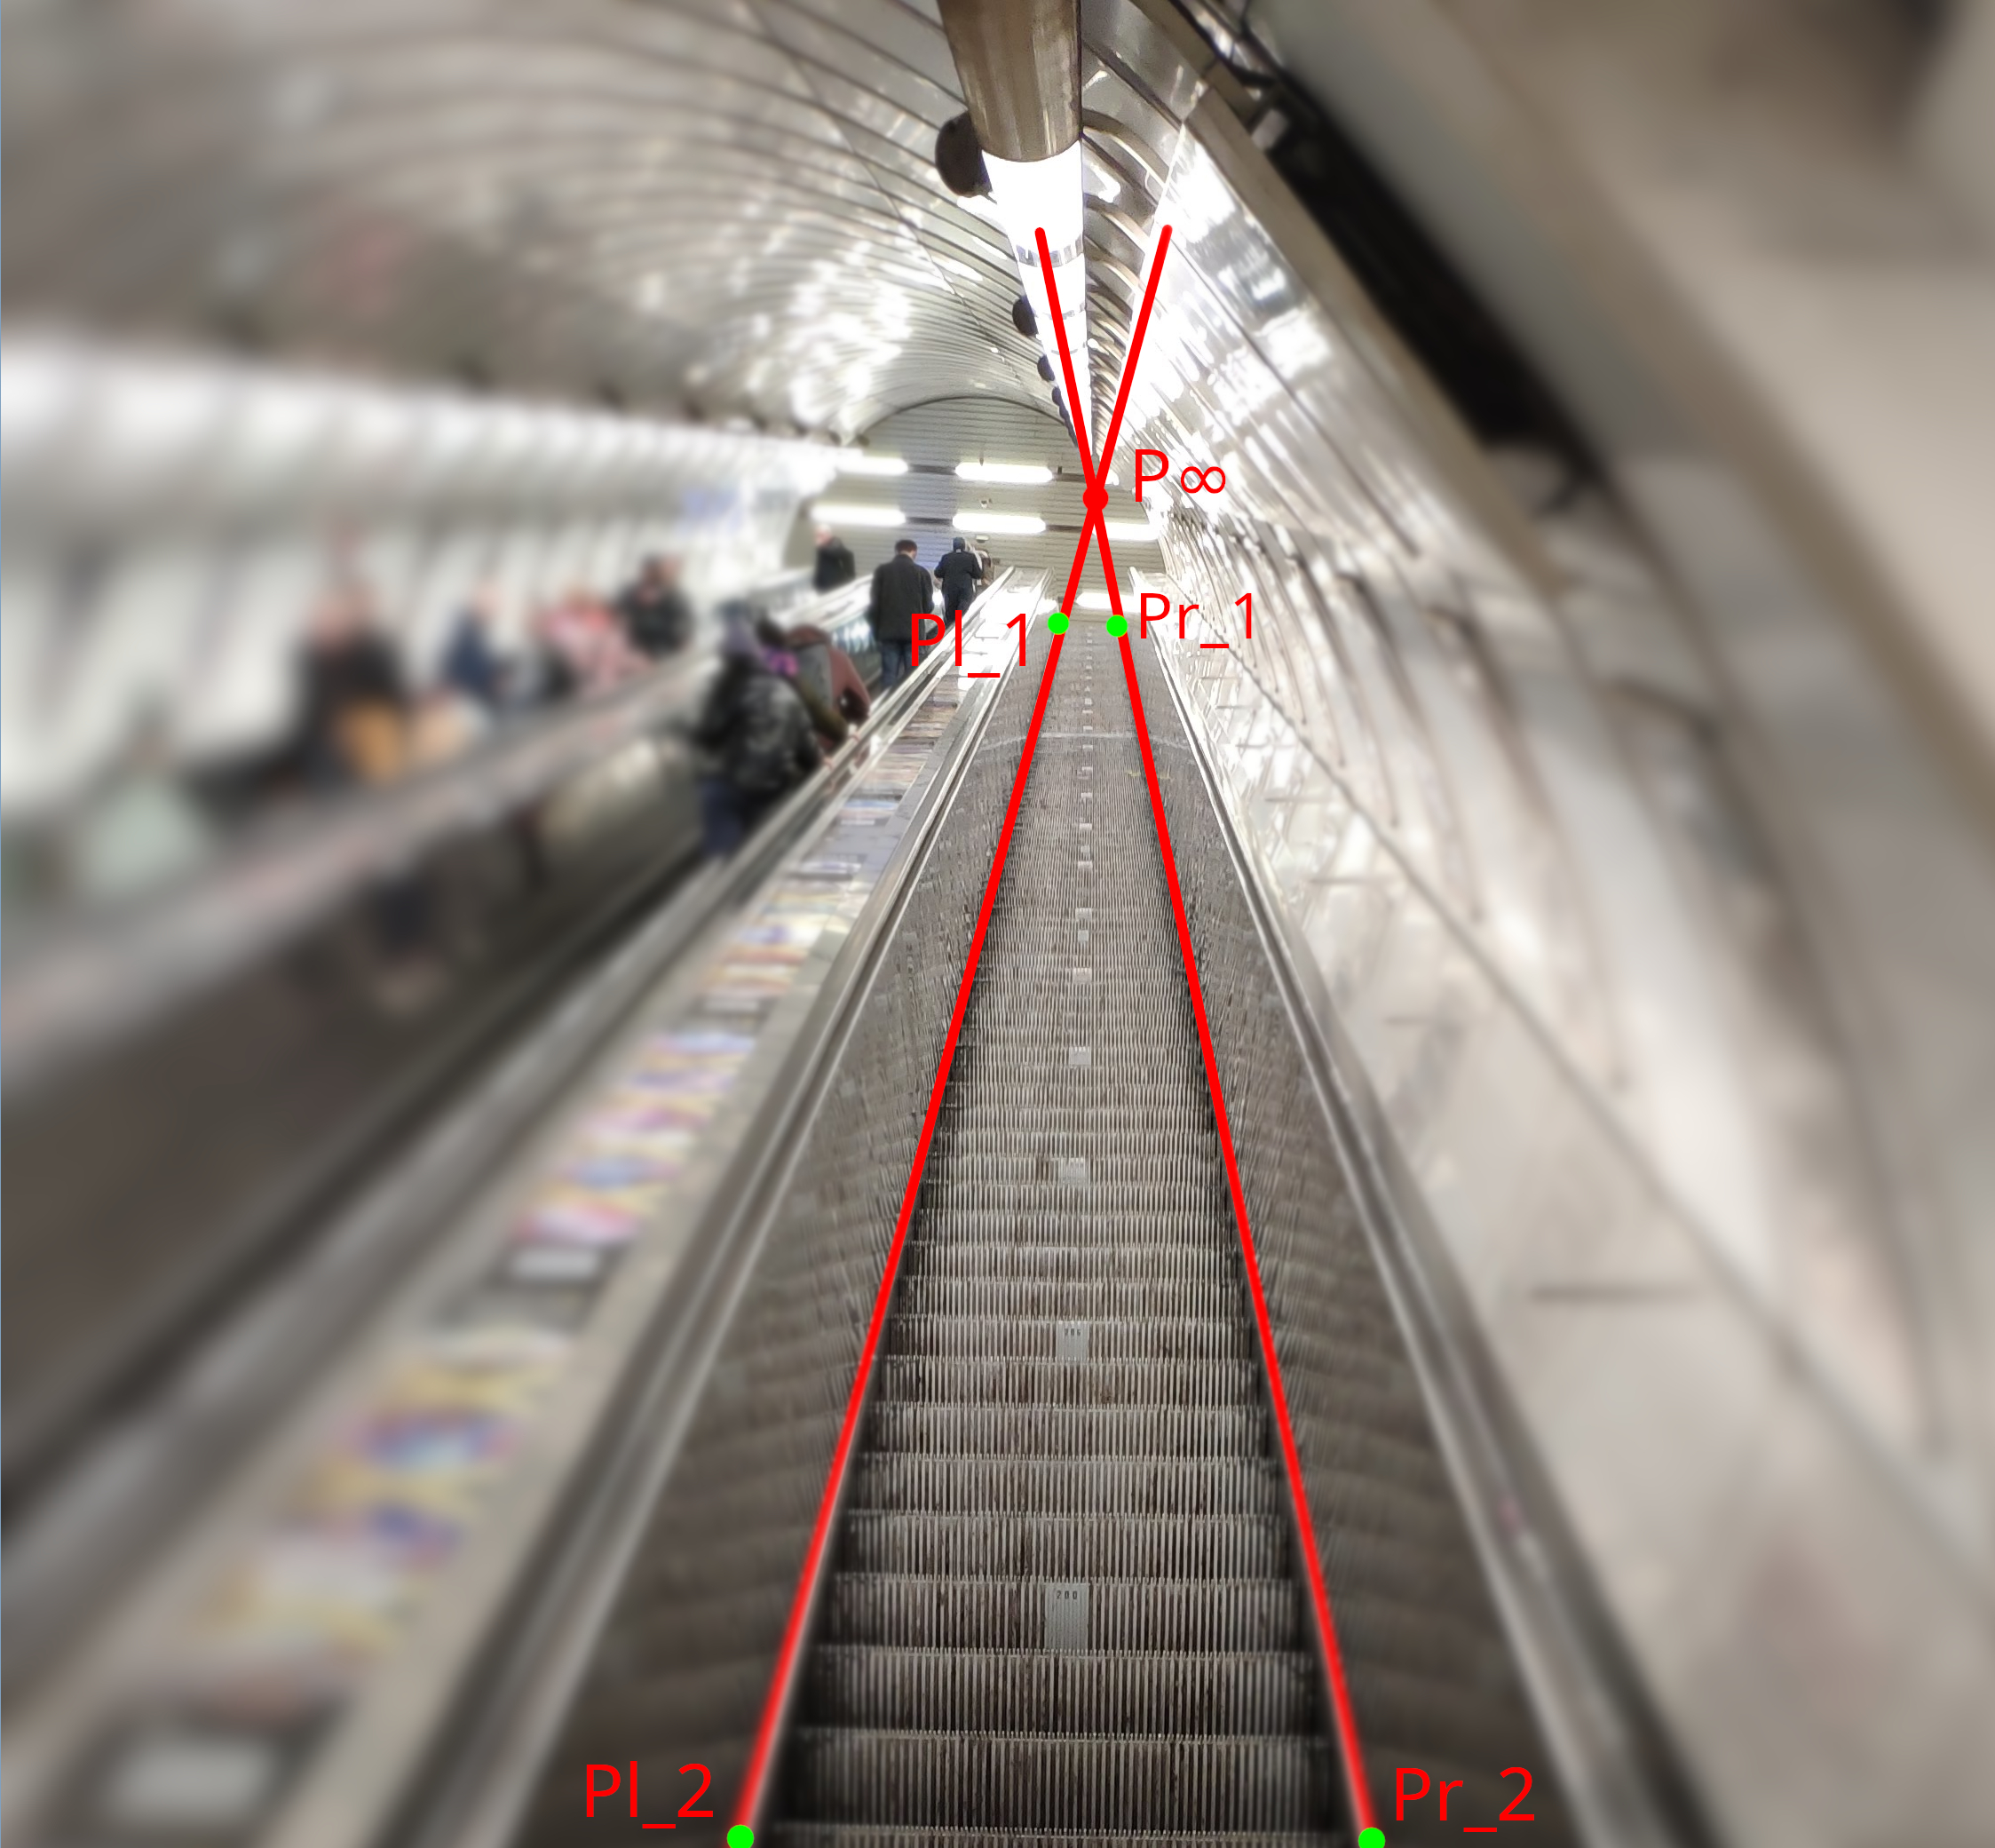
\includegraphics[width=1\textwidth]{graphics/parallel_intersection.jpg}
    \caption{Parallel lines intersection}
    \label{fig:intersection_parallel}
\end{figure}

In Euclidian geometry parallel lines are the lines that have no intersection point. 
In projective geometry, parallel lines are intersecting in a point $x$ at infinity. 
How is it possible? 
In the image \autoref{fig:intersection_parallel} let $l_r = Pr_1 \cap Pr_2 $ and $l_l = Pl_1 \cap Pl_2$. 
In 3D world we know that lines $l_l \parallel l_r$, but after projection on the image plane $\Pi$, we can calculate - in this case even see - the intersecting point $P_{\infty}$. 

Both line and point in a homogenous coordinates can be expressed as vector of three numbers, but if in case of a point homogenous $x = (x, y, z)^T$ will be $m = (\frac{x}{z}, \frac{y}{z})^T$, line $l = (a, b, c)^T$, where $a, b, c$ are parameters of a line equation $ax + by + c = 0$. 
In general case point at infinity is called an \textit{ideal point} and it is not seen on the image, it's coordinates can be expressed as $x_{\infty} = (u, v, 0)^T, \{u, v\} \neq 0$. Same about line - such line is called \textit{ideal line} and it's coordinates are $l = (0, 0, c), c \neq 0$. In algebraic representation, both ideal point and line are lying at the plane $\Pi_0$ (\autoref{fig:homogenous}, green lines).

\begin{figure}[h]
    \centering
    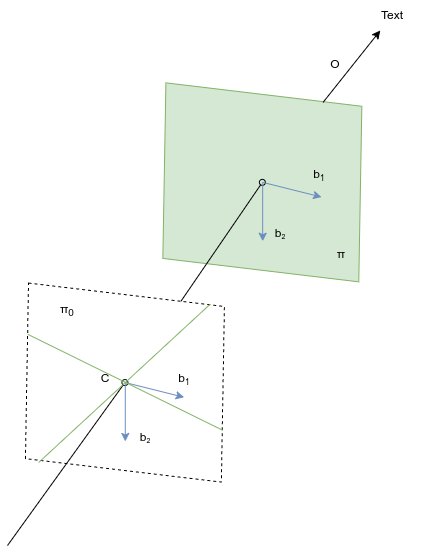
\includegraphics[width=.5\textwidth]{graphics/homogenous.png}
    \caption{Scheme of homogenous coordinates}
    \label{fig:homogenous}
\end{figure}

\section{Pinhole camera model}
Pinhole camera - or a canonical perspective camera model - is a model of a simple camera without optics.
The very first example is a camera obscura - a dark room with a small hole, through which the image from outside is projected on the oposite wall. 
This model can be used to express camera geometry with field of view angles less than $180^{\circ}$.

\subsection{Camera coordinate system}
\begin{figure}[h]
    \centering
    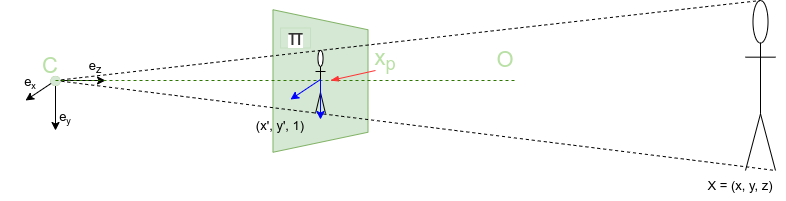
\includegraphics[width=1\textwidth]{graphics/td_scene.png}
    \caption{The pinhole camera model working scheme}
    \label{fig:td_scene_3d}
\end{figure}

\begin{figure}[h]
    \centering
    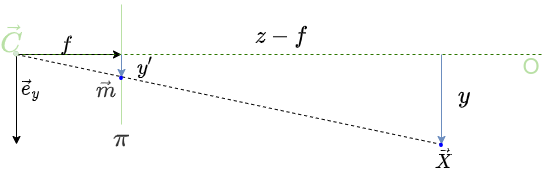
\includegraphics[width=1\textwidth]{graphics/td_scene_yz.png}
    \caption{The pinhole camera model, y-z plane}
    \label{fig:td_scene_yz}
\end{figure}

\begin{figure}[h]
    \centering
    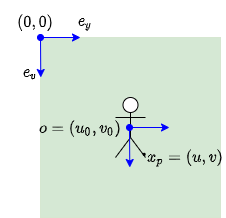
\includegraphics[width=.5\textwidth]{graphics/td_scene_xy.png}
    \caption{The pinhole camera model, x-y plane}
    \label{fig:td_scene_xy}
\end{figure}

In physical implementation of Obscure camera the projective plane is on the oposite side from the Projection center (or Camera center $C$ in pinhole camera model), the image is reversed and mirrored, but in most computer vision literature authors assume that it is on the same side as object (see \autoref{fig:td_scene_3d}).
In \autoref{fig:td_scene_3d} we are looking through a camera with camera center $C$ in a coordinate system with origin at $C$ and basis vectors $(e_x, e_y, e_z)$ on a human. 
Each point $X = (x, y, z)^T$ in a world coordinate system has it's projection $x_p = (x', y', 1)^T$ on a plane $\Pi$ which is located on a distance 1 from a camera center (\autoref{fig:td_scene_yz}). 
Optical axis $O$ is a ray perpendicular to plane $\Pi$, and on the image the point $ O \cap \Pi = x_p$ is a center of the image, see \autoref{fig:td_scene_xy}).

\subsection{Camera calibration matrix}
\begin{figure}[h]
    \centering
    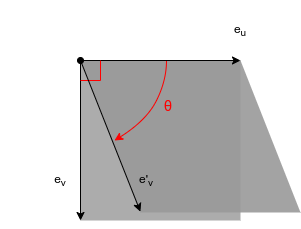
\includegraphics[width=.6\textwidth]{graphics/pixel.png}
    \caption{Scheme of pixel, changing the image (inner) reference frame}
    \label{fig:Kframes}
\end{figure}
Camera calibration matrix - a matrix that includes camera \textit{intrinsic} parameters - pixel size ($e_u$ and $e_v$) and pixel skew angle ($\theta$), as on \autoref{fig:Kframes}, pixel aspect ratio $\bf{a}$ and principle point coordinates $x_p = (u_0, v_0)$.
$$
K = \begin{bmatrix}
    af & -a f cot(\theta) & u_0 \\
    0 & f / sin(\theta) & v_0 \\
    0 & 0 & 1 \\
\end{bmatrix} \hspace{1cm} units: [f]=px, [u_0]=px, [v_0]=px, [a]=1
$$ 
Where $f$ is a focal length used to convert world length ratios to pixels.

In a modern world, every digital camera has a calibration matrix with a square pixel, so in most cases camera matrix looks like:

$$
K = \begin{bmatrix}
    f & 0 & u_0 \\
    0 & f & v_0 \\
    0 & 0 & 1 \\
\end{bmatrix}
$$

\subsection{Projection matrix}

\begin{figure}[h]
    \centering
    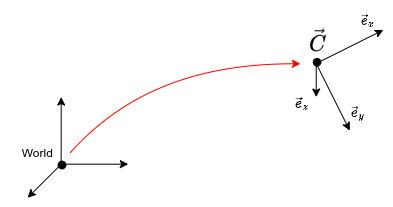
\includegraphics[width=.5\textwidth]{graphics/frames.png}
    \caption{Changing the world (outer) reference frame}
    \label{fig:frames}
\end{figure}
To translate a point from a world coordinate frame to image coordinate frame, Image projection matrix $P$ is used. 
The canonical projection matrix $P_0$ assumes that the camera is in the world coordinate center and that the calibration matrix $K = \bf{I}$
$$
P_0 = \begin{bmatrix} \bf{I} & | & 0 \end{bmatrix} = 
    \begin{bmatrix}
    1 & 0 & 0 & 0 \\
    0 & 1 & 0 & 0 \\
    0 & 0 & 1 & 0 \\
    \end{bmatrix}
$$
But this case is degenerate. 
As far as each camera is different, canonical projection matrix is never used, instead image projection matrix $P$ is used, with applied calibration matrix $K$ to transform canonical $P_0$ to perspective $P$:

$$
P = \bf{K} \begin{bmatrix} \bf{I} & | & 0 \end{bmatrix} = 
    \begin{bmatrix} 
    f & 0 & u_0 & 0 \\
    0 & f & v_0 & 0 \\ 
    0 & 0 & 1 & 0 \\
    \end{bmatrix}
$$

But not always the world coordinate center is located at point $C$ \autoref{fig:frames}. 
Usually it is rotated using a rotation matrix $R$ and translated on vector $t$ where $R$ is a $3x3$ matrix with $det(R) = 1$ and $R^{-1} = R^T$. 
So in general case:

$$
P =   K \begin{bmatrix} \bf{R} & | & \vec{\bf{t}} \end{bmatrix} = 
        K \begin{bmatrix} \bf{R} & | & - \bf{R} \bf{C} \end{bmatrix}
$$
where $C$ is quite often used as a camera position in a world reference frame. 
So matrix $P$ has 6 intrinsic parameters: 3 Euler angles and 3 translation components. 

\subsection{Projection equation}

Image point $m = (u, v)^T$ can be obtained from a point $X$ using $P$ 

$$
\lambda \begin{bmatrix} 
    u \\ v \\ 1 \end{bmatrix} = P \begin{bmatrix} x \\ y \\ z \\ 1
\end{bmatrix}
$$
$$
\lambda \begin{bmatrix} 
    \vec{m} \\ 1 \end{bmatrix} = P \begin{bmatrix} \vec{X} \\ 1
    \end{bmatrix}
$$
Where $\lambda \neq 0$

\section{Epipolar geometry}

\subsection{Skew-symmetric 3x3 matrix}
From \cite{hartley_zisserman_2004}, p.581.


Skew-symmetric or antisymetric matrix is such matrix $[b]_{\times}$ that $[b]_{\times}^T = -[b]_{\times}$. 
For vector $b = (b_1, b_2, b_3)^T$:

$$
[b]_{\times} = \begin{bmatrix}
    0 & -b_3 & b_2 \\ 
    b_3 & 0 & b_1 \\ 
    -b_2 & b_1 & 0 \\ 
\end{bmatrix}
$$
This matrix has some important properties, but the most important in this thesis - it generalizes a cross product as a matrix multiplication
$$
a \times b = [a]_{\times} b
$$

\subsection{Epipolar geometry}
\begin{figure}[h]
    \centering
    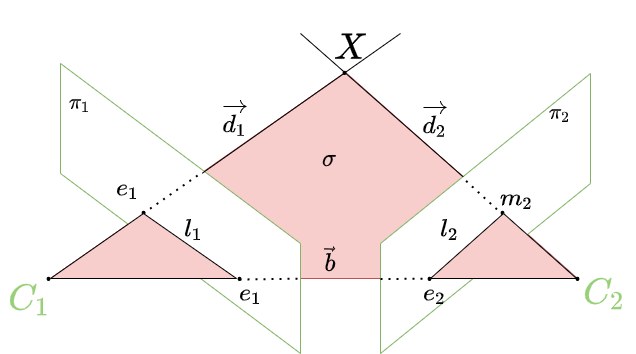
\includegraphics[width=1\textwidth]{graphics/epipolar.png}
    \caption{Epipolar geometry scheme}
    \label{fig:epipolar_std}
\end{figure}
\autoref{fig:epipolar_std} shows a scheme of two cameras with different camera centers $C_1$ and $C_2$ connected with a base line $b = C_2 - C_1$. 
Both of them are seen some 3d point $X$. 
This point projections are $m_1$ and $m_2$ respectivly. 
Points $C_1, C_2$ and $X$ form an \textit{epipolar plane} $\sigma$.
$\sigma \cap \pi_1 = l_1$ and $\sigma \cap \pi_2 = l_2$ are images of \textit{epipolar lines}. 
Epipolar line $l_1$ passes through \textit{epipole} $e_1$, where $\lambda [e_1 | 1]^T = P_2 C_1$, respectivly $\lambda [e_2 | 1]^T = P_1 C_2$.

\subsection{Epipolar constraint}
Having a set of two cameras the relationship between them and constraints on them can be expressed by two new matrices: 
\textit{Essential matrix} $E \in \mathbb{R}^{3x3}, rank(E) = 2$
$$
E = R_2 [C_2 - C_1]_{\times} R_1^T = [-t_{21}]_{\times}R_{21}
$$ 
and \textit{Fundamental matrix} $F \in \mathbb{R}^{3x3}, rank(F) = 2$
$$
F = K_2^{-T} R_2 [C_2 - C_1]_{\times} R_1^T K_1^{-1} = K_2^{-T} [-t_{21}]_{\times} R_{21} K_1^{-1} = K_2^{-T} E K_1^{-1}
$$
where 
$R_{21} = R_2 R_1^T$ is a relative camera rotation and 
$t_{21} = -R_2 b = t_2 - R_{21}t_1$ is a relative camera translation.
The translation $t_{21}$ is lost since E is homogenous.
Epipolar constraint looks like
$$
\begin{bmatrix} m_2 & | & 1 \end{bmatrix} F \begin{bmatrix} m_1 \\ 1 \end{bmatrix} = 0
$$
$F$ maps points to lines, such as
$$
\lambda l_1 = F^T \begin{bmatrix} m_2 \\ 1 \end{bmatrix}
$$
$$
\lambda l_2 = F \begin{bmatrix} m_1 \\ 1 \end{bmatrix}
$$
Also some other properties of $F$ matrix:
$$
F \begin{bmatrix} e_1 \\ 1 \end{bmatrix} = F^T \begin{bmatrix} e_2 \\ 1 \end{bmatrix} = 0
$$

\clearpage
\chapter{Calibration}
\label{chapter:calibration}

\section{Camera calibration}

Camera calibration - computing the camera intrinsic matrix.

\section{Stereopair calibration}

\clearpage
\chapter{Conclusion}
\label{chapter:conclusion}

% Here the proposed algorithm can help - it gives common points to an algorithm, so instead of SfM from 2 images it does SfM from 4 images but with bigger pressision, because $T_{static}$ remains the same, and the only necessary transformation that should be estimated is $T_{t_0t_1}$, and the innertial module can help with that.

% Another possible approach is to use already working SfM algorithm implementation for a left and rigth camera separately to obtaine two pointclouds, and then align them and fix a scale using Iterative closest point algorithm with respect to fixed red pointcloud
\clearpage

%\include{Chapters/Chapter3}
%\include{Chapters/Chapter4} 
%\include{Chapters/Chapter5} 

%----------------------------------------------------------------------------------------
%	THESIS CONTENT - APPENDICES
%----------------------------------------------------------------------------------------

\appendix % Cue to tell LaTeX that the following "chapters" are Appendices

% Include the appendices of the thesis as separate files from the Appendices folder
% Uncomment the lines as you write the Appendices

% \include{Appendices/AppendixA}
%\include{Appendices/AppendixB}
%\include{Appendices/AppendixC}

%----------------------------------------------------------------------------------------
%	BIBLIOGRAPHY
%----------------------------------------------------------------------------------------

% \printbibliography[heading=bibintoc]


\bibliography{main}{}
\bibliographystyle{ieeetr}
\cleardoublepage

%----------------------------------------------------------------------------------------

\end{document}  
